\documentclass[UTF8]{ctexart}
\usepackage{amsmath,amssymb}
\usepackage{tikz}
\usetikzlibrary{calendar}
\ctexset{
    section/format += \sffamily,
    subsection/format += \sffamily,
}
\begin{document}
    \title{\sffamily Log Creative 个人主页开发}
    \author{Log Creative}
    \maketitle
    
    \begin{quotation}
        \noindent \centering \LARGE \emph{学习大前端}
    \end{quotation}
    
    \section{日程安排}

    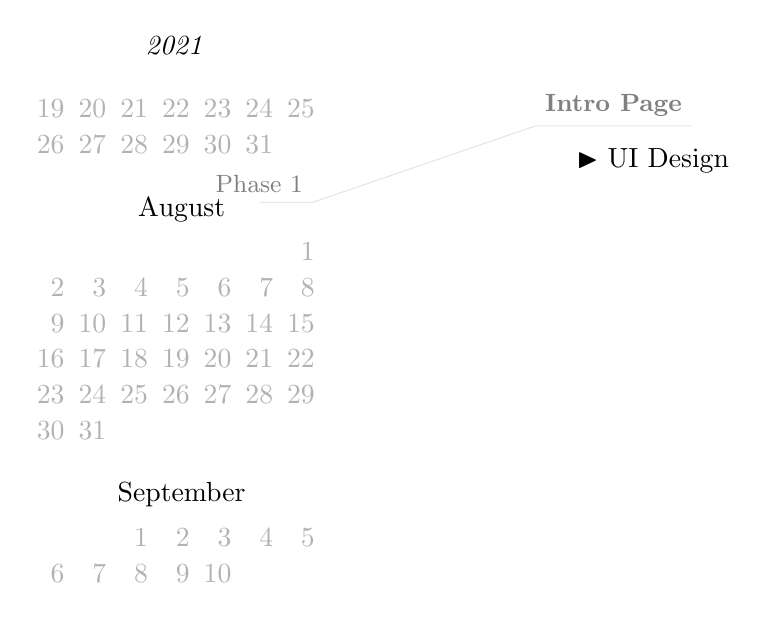
\begin{tikzpicture}[node distance=0.5cm]
        \tikzstyle{note} = [font=\small, black!50];
        \tikzstyle{content} = [note, xshift=4cm, yshift=0.5cm];
        \tikzstyle{noteline} = [black!10];
        \tikzstyle{detail} = [xshift=0.5cm,yshift=-0.2cm];
        \calendar (cal) [
            dates=2021-07-19 to 2021-09-10, 
            week list, 
            month label above centered
        ]   if (Saturday, Sunday) [red]
            if (at most=\year-\month-\day) [black!30]
            if (equals=\year-\month-\day) [blue];
        \node [above of=cal-2021-07-22, node distance=0.8cm] {\emph{2021}};

        \node [below of=cal-2021-07-31,note] (p1n) {Phase 1};
        \node [right of=cal-2021-07-31,content] (p1c) {\textbf{Intro Page}};
        \draw [noteline] (p1n.south) -- (p1n.south east) -- (p1c.south west) -- (p1c.south east);
        \node [below of=p1c,detail] {
            $\blacktriangleright$ UI Design
        };
    \end{tikzpicture}
    
    大部分工作在开学前进行,所有工作的完成不得迟于 10 月。

    预计开播于 7 月 23 日(五),正在进行设备与内容准备。此后每周工作日三个上午 9:00 -- 11:00 直播,视外界环境情形可能会有日程变动。
\end{document}